\documentclass[notes, xcolor=dvipsnames]{beamer}

\usetheme{Warsaw}

\usepackage{inputenc}
\usepackage{graphicx}
\usepackage{amsmath}
\usepackage{amsthm}

\newcommand{\po}{\textcolor{BlueViolet}{po}}
\newcommand{\rf}{\textcolor{Green}{rf}}
\newcommand{\co}{\textcolor{BurntOrange}{co}}
\newcommand{\mo}{\textcolor{Red}{mo}}
\newcommand{\hb}{\textcolor{NavyBlue}{hb}}
\newcommand{\rb}{\textcolor{RubineRed}{rb}}
\newcommand{\xhb}{\textcolor{NavyBlue}{xhb}}
\newcommand{\rfe}{\textcolor{Green}{rfe}}
\newcommand{\rfi}{\textcolor{Green}{rfi}}
\newcommand{\sw}{\textcolor{BurntOrange}{sw}}
\newcommand{\jhb}{\textcolor{NavyBlue}{jhb}}
\newcommand{\jmo}{\textcolor{Red}{jmo}}
\newcommand{\rmo}{\textcolor{Red}{rmo}}
\newcommand{\eco}{\textcolor{WildStrawberry}{eco}}


\title{Understanding POWER Multiprocessors}
\subtitle{Sushmit Sarkar, Peter Sewell, Jade Alglave, Luc Maranget, Derek Williams}

\author{Presented by \\ Akshay Gopalakrishnan}

\begin{document}
    
    \begin{frame}

        \maketitle

    \end{frame}

    \begin{frame}{Introduction}

        \begin{itemize}
            \item Much of the performance in hardware comes due to features such as Read/Write buffers, Speculation, Caches, etc.
            \item The behavior of execution of programs utilizing all such features in a hardware can be defined by a relaxed memory consistency model.
            \item ARM, x86, POWER.. all these hardware exhibit relaxed behaviors.
            \item Of these POWER is relatively well understood.
            \item Major reason is due to informal specification and behaviors described only via litmus tests. 
            \item Continual hardware improvements in POWER also have resulted in more relaxed behaviors.
        \end{itemize}

    \end{frame}

    \begin{frame}{Goal}

        \begin{itemize}
            \item This paper analyzes the POWER multiprocessor family for relaxed behaviors explain their discovered behaviors via an Abstract Machine.
            \item This helps in avoiding getting involved in the complexities of hardware itself while all the way understanding the weak beahviors exhibited by them.
            \item The abstract machine has only one storage subsystem while having read/write buffers for each thread.
        \end{itemize}
        
    \end{frame}

    %Start with some preliminary definitions of orders 
    \begin{frame}{Preliminary Definitions}

        Axiomatic events 
        \begin{itemize}
            \item Read - $R[x]$
            \item Write - $W[x]$
        \end{itemize}

        Binary Relations 
        \begin{itemize}
            \item Program order - $\po$ (per thread syntactic order)
            \item Reads from - $\rf$ (from a write to a read whose value is the write)
        \end{itemize}
        
    \end{frame}

    \begin{frame}{Example 1: Message Passing}

        \begin{figure}
            \makebox[\textwidth][c]{
                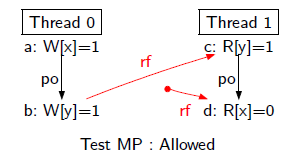
\includegraphics{MP.PNG}
            }
        \end{figure}

        The outcome in program is not allowed under sequential execution, but in POWER such an outcome is allowed.
        In real program, the read to $y$ can be in a loop, which only ends once it reads $1$, indicating that the value of $x$ has been modified.
        But this behavior should then clearly not be possible. But it is.

    \end{frame}

    \begin{frame}{Example 2: Store Buffering}
        
        \begin{figure}
            \makebox[\textwidth][c]{
                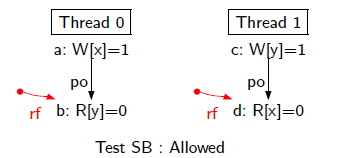
\includegraphics{SB.PNG}
            }
        \end{figure}

        Similarly the outcome in the program above is also allowed under POWER.
        Such an outcome is also observable in x86-TSO.

    \end{frame}

    \begin{frame}{Example 3: IRIW}

        POWER also allows writes to be non-multi-copy-atomic (nmca). 
        Meaning writes can be visible to processors in different orders. 
        The following example showcases an outcome that should not be possible in multi-copy-atomic hardware.
        \begin{figure}
            \makebox[\textwidth][c]{
                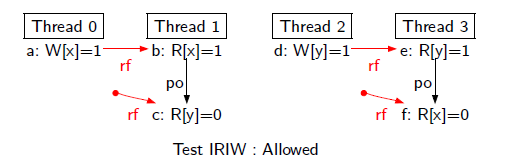
\includegraphics{IRIW.PNG}
            }
        \end{figure}

    \end{frame}

    \begin{frame}{Example 4: WRC }

        Another flavor of nmca is the following example 
        \begin{figure}
            \makebox[\textwidth][c]{
                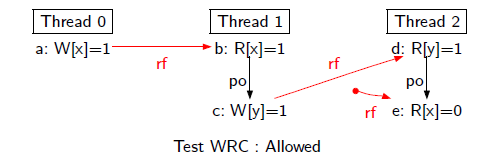
\includegraphics{WRC.PNG}
            }
        \end{figure}
        In this example, the read value of $x$ is $1$, meaning the write has been propagated to Thread 1. 
        Subsequently, Thread 2 reads from a write $\po$ after the read to $x$ in Thread 1. 
        However, this does not ensure that Thread 2 has also received the updated value of $x$.
        The outcome above is allowed in POWER. 

        
    \end{frame}

    \begin{frame}{Use of Synchronization and other Barriers}
        
        The above behaviors of programs may not be desirable in all situations. 
        To ensure this, POWER also comes with barrier instructions: mainly $sync$ and $lwsync$.
        Let us see how these barriers can be used to ensure ordering constraints. 

    \end{frame}

    %From here on the examples involve sync/data/addr/ctrl dependencies.
    %Make sure to understand their differences to observe the examples in detail.
    \begin{frame}{MP + sync}
        
    \end{frame}



\end{document}